% ============================================================
%  SCHOLA DOMESTICA — Level 1, Week 2, Lesson 7
%  Topic: Numbers 8 and 9
%  8–10 problems | No speed drill | Picture-heavy
%  Compile with XeLaTeX
% ============================================================
\documentclass[12pt,letterpaper]{article}
\usepackage{sd_style}

\renewcommand{\lessonnum}{7}
\renewcommand{\lessonweek}{2}

\begin{document}

\lessonheader{2}{7}{Numbers 8 and 9}

\begin{instructbox}
\noindent\textbf{\color{sd-blue}Instruction} \textit{(read aloud):}\\[4pt]
Today we learn 8 and 9.
Eight is the same as two groups of four.
Nine is just one away from ten — almost there!
\end{instructbox}

\vspace{8pt}
\noindent\textbf{\color{sd-blue}Trace and write:}
\tracerowpair{8}{9}

\goldrule
\noindent\textbf{\color{sd-blue}Practice}
\vspace{6pt}

\prob Count and write the number.\\[6pt]
\hspace{1cm}\onedot\onedot\onedot\onedot\onedot\onedot\onedot\onedot\quad\ansblank

\vspace{10pt}
\prob Count and write the number.\\[6pt]
\hspace{1cm}\onedot\onedot\onedot\onedot\onedot\onedot\onedot\onedot\onedot\quad\ansblank

\vspace{10pt}
\prob How many?\\[4pt]
\hspace{1cm}%
\IfFileExists{stars_8.jpg}{
\includegraphics[height=1.4cm]{stars_8.jpg}}{%
  \onestar\onestar\onestar\onestar\onestar\onestar\onestar\onestar}
\quad\ansblank

\vspace{10pt}
\prob How many?\\[4pt]
\hspace{1cm}%
\IfFileExists{apples_9.jpg}{\includegraphics[height=1.4cm]{apples_9.jpg}}{%
  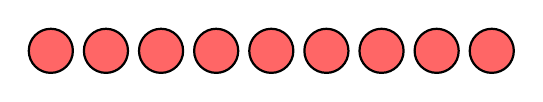
\begin{tikzpicture}[baseline=0]
    \foreach \x in {0,...,8}\draw[fill=red!60,thick](\x*0.7,0)circle(0.28);
  \end{tikzpicture}}
\quad\ansblank

\vspace{10pt}
\prob Circle the group of \textbf{8}.\\[6pt]
\begin{center}
\begin{tabular}{ccc}
\textbf{A}\quad%
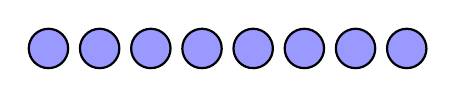
\begin{tikzpicture}[baseline=0]
  \foreach \x in {0,...,7}\draw[fill=blue!40,thick](\x*0.65,0)circle(0.25);
\end{tikzpicture}
&\quad\quad&
\textbf{B}\quad%
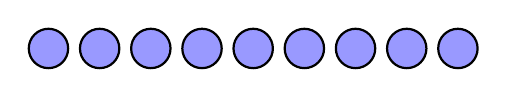
\begin{tikzpicture}[baseline=0]
  \foreach \x in {0,...,8}\draw[fill=blue!40,thick](\x*0.65,0)circle(0.25);
\end{tikzpicture}
\end{tabular}
\end{center}

\vspace{10pt}
\prob Draw \textbf{9} stars in the box.\\[4pt]
\noindent\fbox{\rule{0pt}{2.4cm}\hspace{11cm}}

\vspace{10pt}
\prob \textit{(Teacher reads)} A mouse gathered 5 acorns in the morning
and 3 more in the afternoon.
How many acorns did she gather? \quad\ansblank

\vspace{10pt}
\prob Write the missing numbers:\\[6pt]
\hspace{2cm}{\Large 6 \quad \ansblank \quad 8 \quad \ansblank \quad 10}

\vspace{10pt}
\prob Which is more: 8 or 9? \quad\ansblank

\vspace{10pt}
\prob Which is fewer: 8 or 6? \quad\ansblank

\goldrule

\begin{checkbox}
\noindent\textbf{\color{sd-green}Knowledge Check}\\[4pt]
\setcounter{probnum}{0}
\prob Write the number eight: \quad\ansblank \quad
  Write the number nine: \quad\ansblank\\[8pt]
\prob \onedot\onedot\onedot\onedot\onedot\onedot\onedot\onedot\onedot\quad
  How many? \quad\ansblank
\end{checkbox}

\vfill
\noindent{\color{sd-blue}$\bigstar$ \textbf{Enrichment:}}
In Latin, eight is \textit{octō} and nine is \textit{novem}.
Do you know a word that uses \textit{octo}? \textit{October} was once the eighth month of the Roman calendar!

\vspace{4pt}\hrule\vspace{3pt}
{\footnotesize\color{gray}\textit{Teacher note: Eight (octō) is an excellent hook to Roman/classical vocabulary.
  If the student struggles with 8 vs 9, use dominoes or a ten-frame to show the difference visually.}}

\end{document}
